\section{Implementation}

We have implemented our browser extension in Firefox 69.0. Our signatures are currently stored in a local JavaScript file in the extension package.

\subsection{Loading signatures}
Our network filter/detector loads signatures and finds injection points in the document. However, there might be a large number of signatures which don't need to be loaded for a specific website. For example, if several signatures are designed for pages running a WordPress plugin, then the extension need not check any of these for a site which is not running WordPress at all. On the other hand, if a site is running WordPress, we might have to check all signatures meant for WordPress, but not others. Therefore, when loading signatures, we proceed in a manner similar to a decision tree. The detector first probes the page to identify the underlying framework (we call this the 'software' in our signature language). These are usually found by hints in the document HTML. These probes are framework-specific, and as such, need to be encoded in some way so that the detector can run them. There are two approaches for this: the detector completely takes care of this, and needs to be maintained for changes in frameworks and future technologies, or, the signature developer additionally specifies a more specialized version detector as part of a probe file. We chose to go with the first option, as this provides a greater ease of use for signature developers. In our prototype implementation, hard-coding probes into the detector did not imply a substantial amount of work. However, as more signatures are written and more applications are required to be included, this can become an arduous task. We believe the second option can be desirable and would not be a terrible burden for signature developers: for example, the widely popular network mapping tool Nmap \cite{nMap} uses probes in a similar manner, and these are kept in a modifiable file so that advanced users can have more expressibility. After running these probes, the detector loads signatures for the specific software (e.g. all signatures for WordPress web sites).  

At this point, we filter out the ones that do not apply to the current page by iterating through the list of signatures sequentially. The detector checks whether the identifying information of the signature matches the given HTML string and/or URL.

\subsection{Version identification}
Finally, we apply version identification. Our objective for versioning is that our signatures don't trigger any false positives on websites running patched software. We found this to be one of the harder aspects of signature loading. In WordPress, for example, many of the plugins do not update their file names with the latest versions, or do not include them at all, and thus, this information is often hard to come by from the client-side perspective. In the case of WordPress, the wp-admin/plugins.php subpath contains information about all currently active plugins on the site. Unfortunately, this information is only available to admins of the site. While this might not be the bulk of users, it is, on the other hand, the bulk of disclosed CVEs, as described in Section 4. Furthermore, we believe that even if we load a signature when the application has already been fixed at the server-side, it will often preserve the page's functionality, as many of the CVEs describe XSS which happens as a result of unsanitized input that was not meant to be JavaScript code regardless. Motivated by this observed behaviour, our mechanism follows a series of increasingly accurate but less applicable version identifiers: first, we apply general-purpose version probes, like the one described for WordPress (these are maintained in a similar way to software probes, hard-coded in the detector logic). If these are not successful, the signature language provides functionality for version identification in the HTML through regex. If the developer considers version information to be unavailable through the HTML, the version in the signature is left blank and the detector applies the signature patch regardless of version, as we can not be sure the page is running patched software.

\subsection{Dynamic injections}
Some of the exploits manifest themselves through dynamically loaded files. For example, CVE-2018-7747 had XSS triggered when the user loaded information stored in the plugin's database after clicking on an element of the page. Since this was not loaded with the original HTML, it came as a response to an Ajax request. Our signature language provides functionality to protect against these kinds of exploits, as shown in the example below:

 \lstset{basicstyle=\small}
\begin{lstlisting}
url: 'wp-admin/admin.php?page=caldera-forms',
...
type: 'listener',
listenerData: {
	listenerType: 'xhr',
	listenerMethod: 'POST',
	sanitizer: 'escape',
	type: 'string',
	url: 'wp-admin/admin-ajax.php',
	typeDet: 'single-unique',
	endPoints: ['<p><strong>', '[AltBody]']
}
\end{lstlisting}

This signature describes an exploit on a WordPress site running the Caldera Forms plugin. The XSS occurs in the specified url. The listenerData attribute defines an extra listener to attach in the background page of the extension. In this case, the page listens for an XHR, specifically done as a POST to the specified subdomain listenerUrl. The rest of the information is similar to a regular signature, as it will execute the filter and sanitize the response if necessary, according to the specified endpoints. The background page knows to only filter such requests originated from the correct web page. The type of resource to listen for is taken as specified by the webRequest API. 

\begin{figure}[h]
	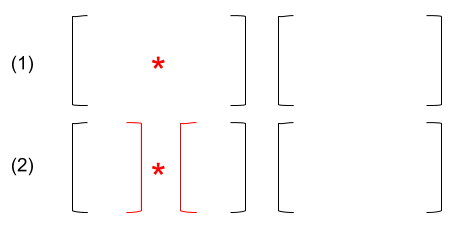
\includegraphics[scale=0.5]{img/attacker_injection_compound.png}
	\caption{Example attacker injection when multiple injection points exist in the page. (1) shows a basic injection pattern. (2) shows an attempt to fool the detector.}
	\label{fig:attacker_injection}
\end{figure}

\subsection{Handling multiple injections in one page}
In the previous example, the endPoints were listed as two strings in the incoming network response. However, there are cases where arbitrarily many injection points can be generated by the php code, such as a for loop generating table rows. For these, it is hard to correctly isolate each endPoint pair, as an attacker could easily inject fake endPoints in between the original ones.

We illustrate one case of this mechanism using Figure~\ref{fig:attacker_injection} as a visual aid: In (1), the content in black is a template. The content in between the brackets is an injection point, where dynamic content is injected into the template. In the case of a vulnerability, the injected content (\textcolor{red}{*}) can expand to any arbitrary string. The signature separates the injection from the rest by matching for the start and end points (called the endPoints), represented by the brackets. This HTML originally has two pairs of endPoint patterns.

In (2), the attacker knows these are being used as injection endPoints and decides to inject a fake ending point and a fake starting point, with some additional malicious content in between (shown in red). If the detector were to look for several pairs of endPoints, it would not be able to tell the difference between the red and black patterns, even when using our top-down, bottom-up approach, and would not be able to get rid of the content injected in the red star (\textcolor{red}{*}). Therefore, we have to use first starting point and the last ending point and sanitize everything in between. Depending on the application, this might get rid of a substantial amount of valid HTML, in particular, the web page's functionality might be affected. Note that due to the difficulty of applying a general solution to this scenario, we defer to the signature developer's judgement, of what behaviour the detector should follow. We expand upon this further in Section 5.


\begin{figure}[h]
	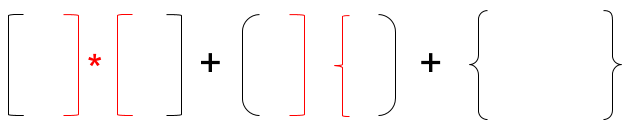
\includegraphics[scale=0.4]{img/attacker_injection_unique.png}
	\caption{Example attacker injection when multiple distinct injection points exist in the page}
	\label{fig:attacker_injection_unqiue}
\end{figure}


Figure ~\ref{fig:attacker_injection_unqiue} illustrates a case when there are several injection points in one page, but each of them is distinct. Now, because the filter is only looking for one pair of brackets, the attacker can't fool the extension into leaving part of the injection unsanitized. However, they could inject an extra ending bracket after the opening parenthesis, or similarly, an extra opening brace before the ending parenthesis. In either case, the extension will be tricked into sanitizing non-malicious content, the black pluses (+). We can detect this behaviour by noting that we know the order in which the endPoints should appear, and so if the filter sees a closing endPoint before the next expected starting endPoint, or similarly, a starting endPoint before the next expected closing endPoint, this attack can be identified. In the diagram, the order is brackets, parenthesis, braces. When it sees a closing bracket after an opening parenthesis, and similarly, when it sees an opening brace before a closing parenthesis, this represents the described attack. As with the previous scenario, we can not easily identify which endPoint is the real one, so sanitization will still potentially get rid of non-malicious content. As before, the signature developer specifies whether the page should be blocked or sanitization goes through as usual when this behaviour is detected.

While our prototype's signature database is currently encoded entirely in the extension software, we envision that a trusted entity can maintain this database, such as those that currently maintain CVE databases, and will have to be audited so that it is not filled with false signatures and existing ones are not compromised.